\section{Introduction}
\IEEEPARstart{M}{ulti-target} defense requires a team to protect several assets while the numbers of available defenders and incoming attackers change. A policy trained separately for every deployment population would be costly to maintain. The desired alternative is to train once on small engagements and reuse the same parameters when the team or the set of protected assets grows. Accepting a variable-size observation is necessary for this transfer, but the harder question is what information the policy should extract from that observation.

An attacker's threat is contextual. Its motion matters together with the asset it approaches and the teammates already covering that asset. We call this joint attacker--target--teammate information the \emph{threat context}. Figure~\ref{fig:motivation} illustrates two scenes with the same attacker--target approach geometry. In one, teammates already cover the target; in the other, the acting defender must respond to a coverage gap. The attacker alone does not distinguish these situations. A useful representation should combine target coverage with the approaching threat before the acting defender compresses the scene into its decision feature. With more entities, these relationships occur in new combinations, so the process that constructs the context must be reusable.

\begin{figure*}[!t]
\centering
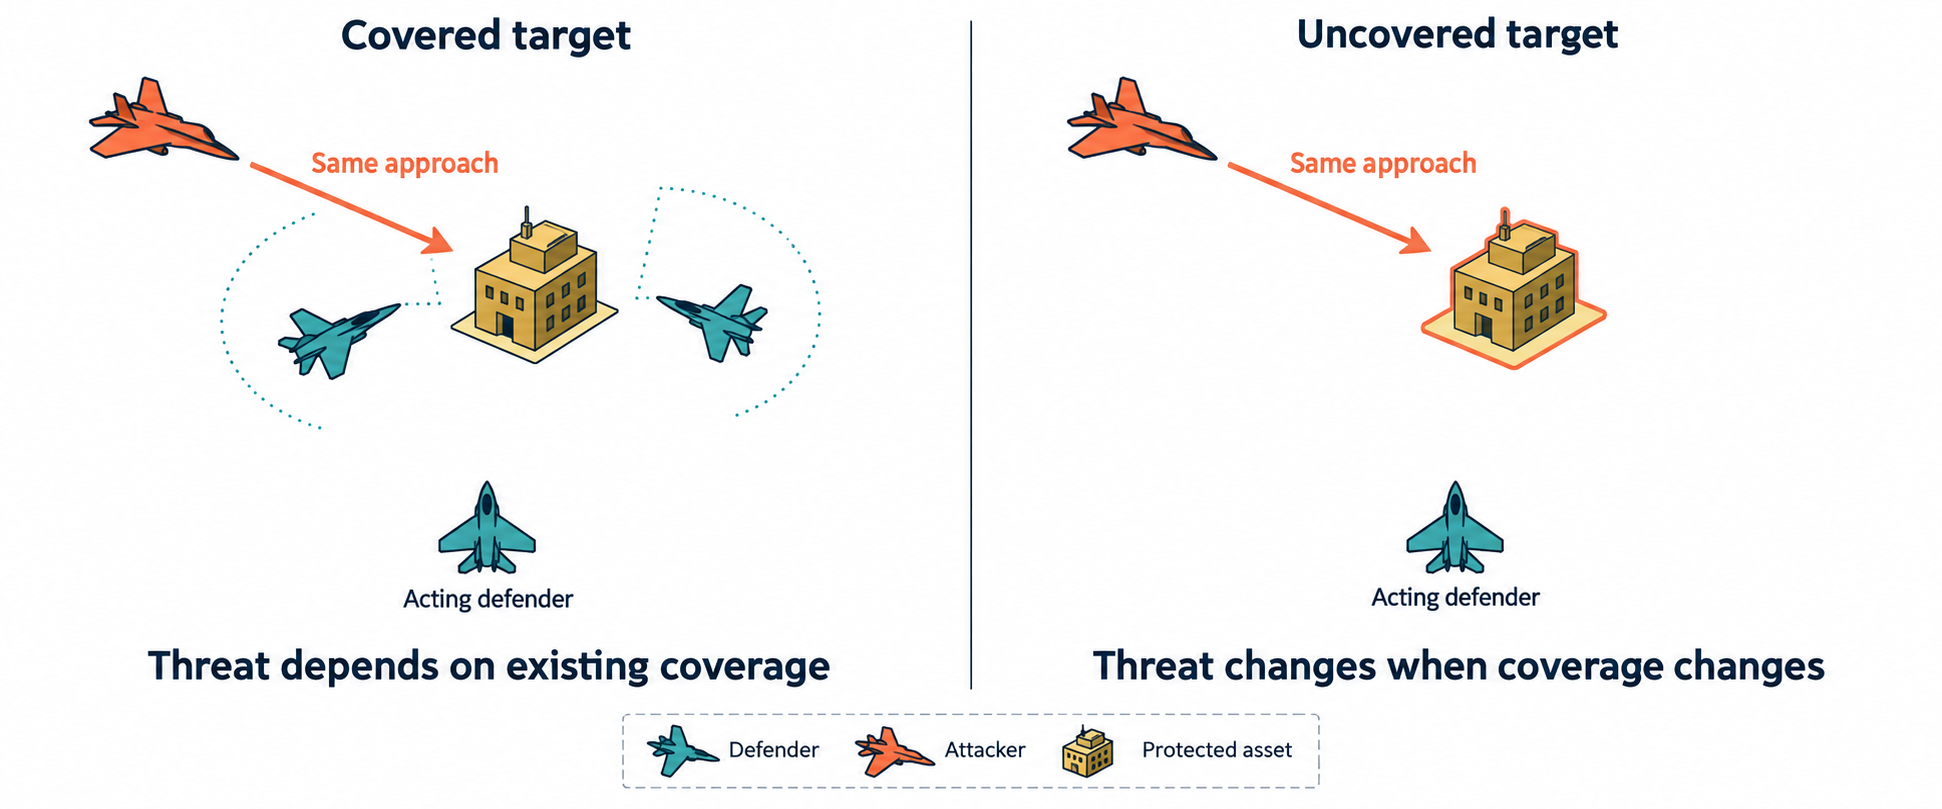
\includegraphics[width=0.92\textwidth]{figures/fig_motivation.png}
\caption{Motivation: matched attacker--target approach geometry can demand a different defensive response when teammate coverage changes. LEAF is designed to build this threat context before receiver-specific reading. The illustration is conceptual; coverage arcs are illustrative and are not simulator measurements.}
\label{fig:motivation}
\end{figure*}

Two further requirements shape the representation. First, the same scene has different implications for a free defender and one already engaged elsewhere. Reading should therefore be conditioned on the acting defender. Second, current scene processing and temporal inference have distinct roles. Attacker intent is not directly observed, so history remains useful for action selection. Yet a recurrent summary learned on small engagements may change distribution as the population grows. Feeding that summary back into every context read exposes scene interpretation to an additional source of shift. This motivates constructing and reading the current context before incorporating recurrent memory.

Existing approaches address parts of this problem. Differential games and task allocation organize interception through geometry, matching, and assignments~\cite{chen2017reachavoid,yan2020barriers,shishika2020perimeter}. Their guarantees rely on the chosen dynamics and task structure. Entity-based cooperative learning supports variable populations~\cite{iqbal2021refil,park2026spectra}, but a single self-to-entity attention read has no explicit intermediate stage for constructing the threat context. Hierarchical allocation, as in ALMA~\cite{iqbal2022alma}, introduces a discrete task organization before maneuvering. Entity Transformers such as UPDeT and TransfQMix~\cite{hu2021updet,transfqmix2023} perform richer interaction and incorporate temporal tokens. Their usual fixed-depth computation does not directly address how one current-scene refinement operator can be reused at different execution depths. Our focus is this organization of context construction, receiver-specific access, and memory.

We propose \textbf{Looped Entity Attention Fusion (LEAF)}. At each physical decision, a shared entity-attention operator repeatedly refines the current entity set. A query derived from the defender's current self representation reads each stage, and learned weights fuse the reads. Training samples the number of rounds, encouraging the same operator to support decisions at several exits. The fused context augments the REFIL feature, after which a temporal GRU incorporates history and produces action values. Parameters are shared across entities, defenders, and refinement rounds. The loop processes one observation; the GRU carries information between observations.

We evaluate frozen policies in SkyHAD after training only with at most ten vehicles per team and three targets. Deployment reaches fifty vehicles per team or twelve targets, with separate target-count, team-size, and joint extrapolation groups. LEAF has lower mean target damage than all compared learned baselines and the rule-based controller in each group. The experiments then distinguish three questions: whether the overall policy transfers, which design changes affect transfer, and how the frozen policy uses its refinement stages. The one-round exit of a multi-depth-trained LEAF remains effective even though a separately trained one-round model transfers less well on average. Execution through six rounds, beyond the training maximum of four, gives similar aggregate damage. These observations support reusable refinement over the evaluated range without assuming that more computation must always help.

Our contributions are:
\begin{enumerate}
\item A threat-context encoder combining shared iterative entity updates, current-state receiver queries, and stage fusion before temporal memory, integrated with cooperative value learning.
\item Structural analysis of permutation consistency and a finite-depth action-stability bound, clarifying what the architecture guarantees and what remains an empirical generalization claim.
\item A unified experimental account comprising baseline comparisons, seven trained design variants, and frozen-policy mechanism studies, connecting population transfer to depth robustness, intermediate reading, and target-protection behavior.
\end{enumerate}
